\documentclass[12pt,a4paper]{article}

\usepackage[a4paper, top = 2cm, bottom = 2cm, left = 1.5cm, right = 1.5cm]{geometry}
\usepackage[dvipsnames]{xcolor} % Colors

\usepackage{standalone}

\usepackage{setspace}
\usepackage{graphicx}
\usepackage{amsfonts}
\usepackage{amsmath}
\usepackage{tikz}
\usepackage{pdfpages}
\usepackage{epigraph}
\usepackage{csquotes}

% Bibliography
\usepackage{xcolor}
\usepackage{hyperref}
\hypersetup{
    colorlinks=true,
    citecolor=MidnightBlue,
		linkcolor=MidnightBlue,
    pdfpagemode=FullScreen,
    }

\usepackage{natbib}
\usepackage[noabbrev]{cleveref}
\setcitestyle{authoryear,open={(},close={)}}
\bibliographystyle{plainnat}

\usepackage{subfiles}

\setlength\parindent{0pt}
\spacing{1.2}
%%%%%%%%%%%%%%%%%%%%%%%%%%%%%%%%%%%%%%%%%%%%%%%%%%%%%%%%%%%%%%%%%%%%%%%%%%%%%
\begin{document}

\section*{Exercise 2}

\textbf{Q: Why do I ask you to choose such a high degree of risk aversion?}
A: While theta between 1 and 4 is a reasonable number for usual economic applications, it makes the optimal share invested in the risky asset skyrocket.. I.e. if we want realistic investment choices over the lifecycle, we need a very high degree of risk aversion \\ \\

\textbf{Q: What does it mean that $\alpha_t > 1$ for young ages? }
A: We want to buy more risky assets than affordable, i.e. we want to short them? (Shorting = borrow them and sell them on the market?) \\ \\

\textbf{Q: How does the optimal portfolio share $\alpha_t$ vary with theta? }
A: Note, that alpha varies with thata the same way as $\alpha_hat$ varies with theta, as $\alpha = \alpha_hat * (W_t - C_t)/ (X_t - C_t)$ \\ \\

\textbf{Q: What are the properties of consumption over the life-cycle and how do you interpret this path in light of the data features mentioned in the lecture?}
A: \\ \\


\textbf{Q: Simulate the model under three settings:}\\
\textbf{(a) rho = 0.02, tetta=150}\\
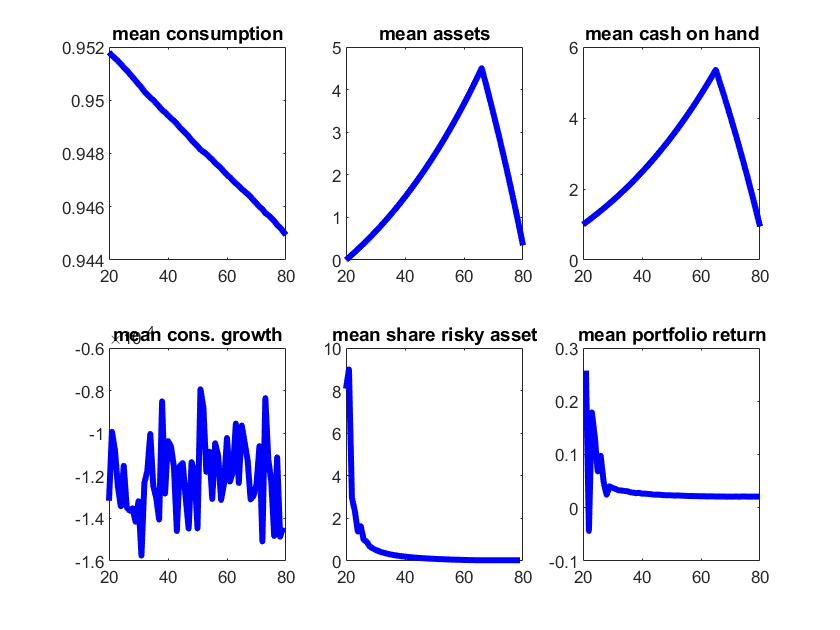
\includegraphics[width = 0.9\textwidth]{PS3/rho0.02tetta150.png}
\\
\textbf{(b) rho = 0.02, tetta=200} \\
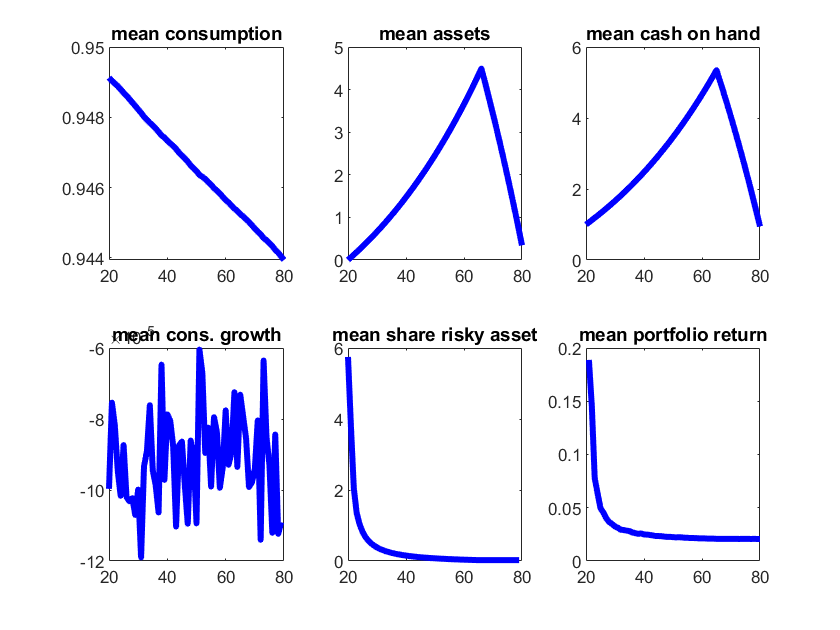
\includegraphics[width = 0.9\textwidth]{PS3/rho0.02tetta200.png}
\\
\textbf{(c) rho = 0.04, tetta=150} \\
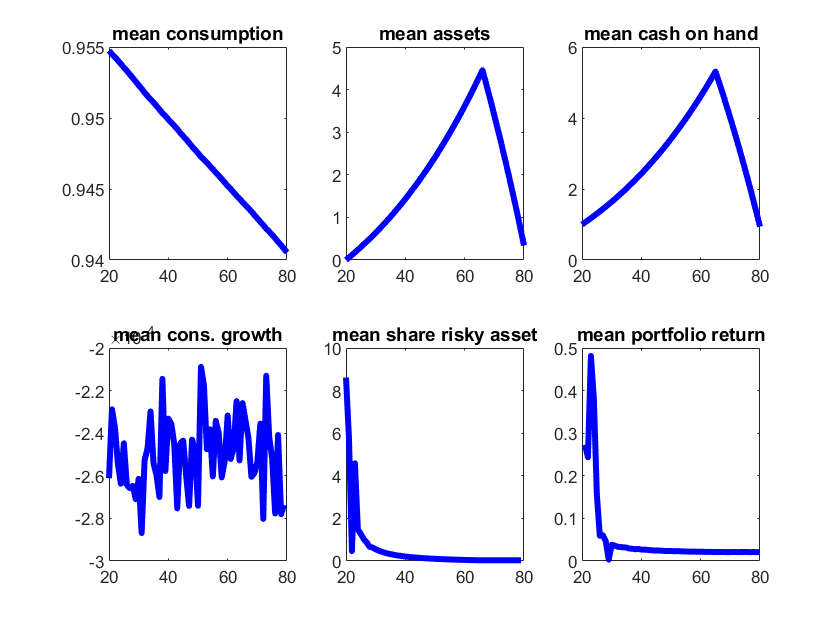
\includegraphics[width = 0.9\textwidth]{PS3/rho0.04tetta150.png}
\\


\section*{Problem 3}
\textbf{Q: Relate the portfolio allocation for the case $\theta = 150$ and $\rho = 0.04$ to the "rule of thumb" advice of a fund manager who suggests to hold $\alpha_j = 1- \frac{j}{100}$ in stocks where $j$ is age.}

Here $\rho$ is chosen to be rather large, leading to a lower $\beta$. This means, that people are more impatient and care relatively more about current consumption (or, expressed differently, care relatively less about future consumption).

Below, there is a graph comparing the recommended share in the risky asset to the estimated model prediction (obviously, this is based on our assumptions about how the returns/ incomes behave).

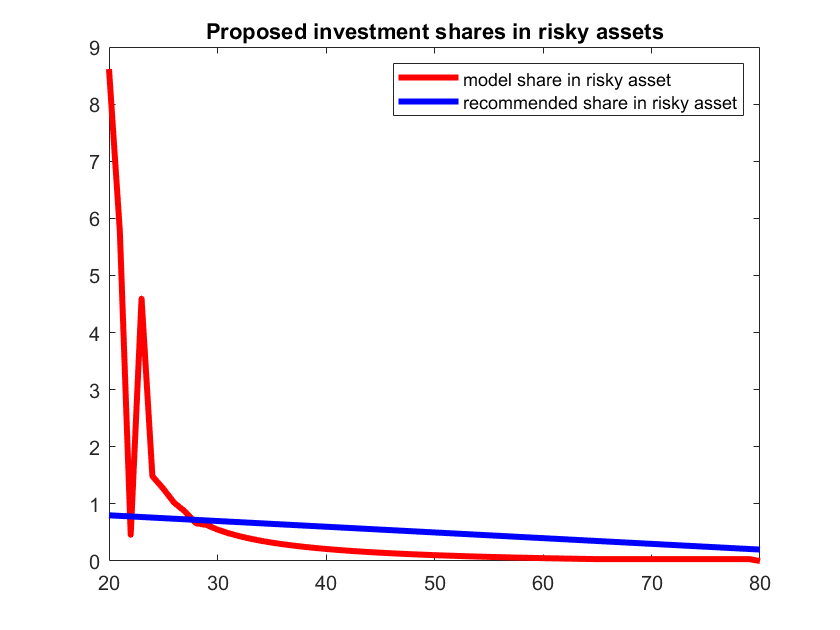
\includegraphics[width = 0.9\textwidth]{PS3/sharesriskyasset.png}
\\
When we run the simulation \textbf{n = 100,000 times} the spike around age 23 becomes less negative\\
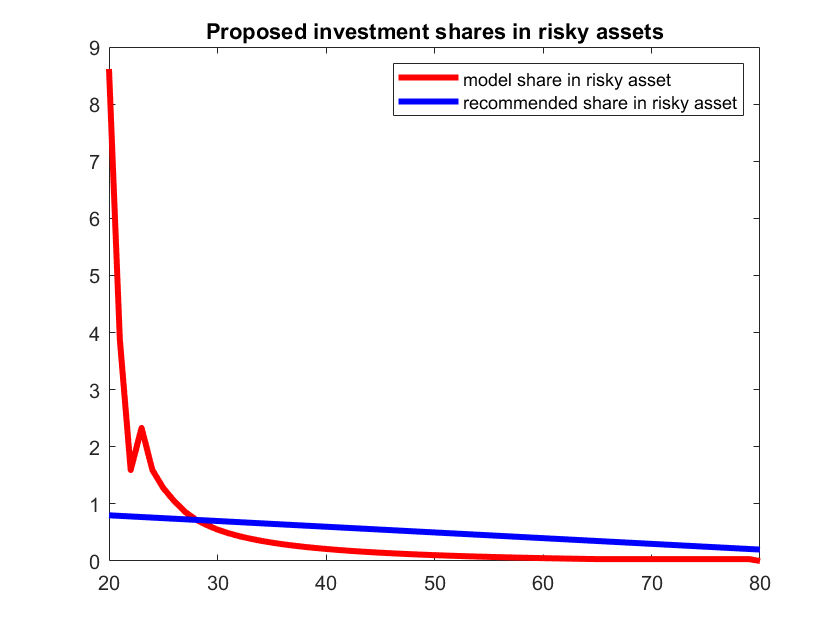
\includegraphics[width = 0.9\textwidth]{PS3/sharesriskyassetns100000.png}
This indicates, that the optimal shares predicted by the model will smooth out when n converges to infinity!
\end{document}